\documentclass{beamer}
\usetheme{Warsaw}

\usepackage[arrow,curve,matrix,frame]{xy}

\newcommand{\<}{\langle}
\renewcommand{\>}{\rangle}

\title{Weighted Finite State Transducers}
\author{Ilya Edrenkin and Georgy Bronnikov}
\date{October 24, 2012}

\begin{document}

\maketitle

\section{Definitions and preliminaries}

\begin{frame}
  \begin{itemize}
  \item Finite State Automaton (FSA)
    \begin{itemize}
    \item definition
    \item main applications
    \end{itemize}
  \item Weighted Finite State Automaton (WFSA)
    \begin{itemize}
    \item definition
    \end{itemize}
  \item Finite State Transduser (FST)
    \begin{itemize}
    \item definition
    \end{itemize}
  \item Weighted Finite State Transducer (WFST)
    \begin{itemize}
    \item definition
    \item advantages over WFSA
      \begin{itemize}
      \item composability
      \item invertibility
      \end{itemize}
    \item equivalence
    \end{itemize}
  \item Digression: Semirings
    \begin{itemize}
    \item definitions
    \item examples
    \end{itemize}
  \end{itemize}
\end{frame}

\section{Basic component WFSTs used in speech recognition}

\begin{frame}
  \frametitle{Acoustic model}

  $$
  \begin{xy}
    \entrymodifiers={++[o][F-]}
    \xymatrix@C=2cm{
      {1} \ar[r]^{\mbox{d1}:a/0.5}
      \ar@(ur,ul)[ud]_{\mbox{d1}:\epsilon/0.5}& 2
      \ar[r]^{\mbox{d2}:\epsilon/0.5}
      \ar@(ur,ul)[ud]_{\mbox{d2}:\epsilon/0.5} & 3
      \ar[r]^{\mbox{d3}:\epsilon/0.5}
      \ar@(ur,ul)[ud]_{\mbox{d3}:\epsilon/0.5} & *++[o][F=]{4} 
    }
  \end{xy}
  $$

\end{frame}

\begin{frame}
  \frametitle{Lexicon}

  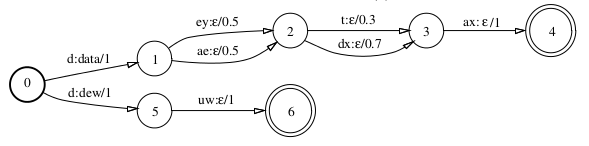
\includegraphics[width=9cm]{lexical-transducer.png}

  Mohri et al. claim that lexical items should be output at the
  starting nodes of the phonetic segments that correspond to them.
\end{frame}

\begin{frame}
  \frametitle{Grammar}

  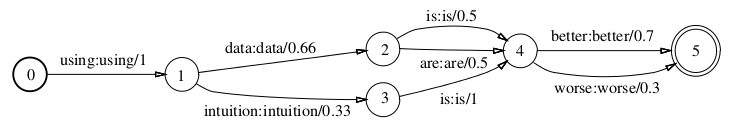
\includegraphics[width=9cm]{grammar-transducer.png}
\end{frame}

\section{WFST production algorithms}

\subsection{Composition}

\begin{frame}
  \frametitle{Composition}

  Given a WFST $T_1$ from input alphabet $\mathcal{A}$ to output alphabet
  $\mathcal{B}$, and $T_2$ from $\mathcal{B}$ to $\mathcal{C}$, produce a WFST $T_1 \circ
  T_2$ from $\mathcal{A}$ to $\mathcal{C}$, such that the results of applying $T_1
  \circ T_2$ to a string $s \in \mathcal{A}^*$ is equivalent to the results of
  first applying $T_1$ to the same string, then running $T_2$ over the
  results (the same output strings receive the same weight).
\end{frame}

\begin{frame}
  \frametitle{The case without empty transitions}

  Basically, a cartesian product of the two transducers.

  Let 
$$
\begin{array}{ll}
T_1 = \<\mathcal{A}, \mathcal{B}, Q_1, I_1, F_1, E_1, \lambda_1, \rho_1\> &
  \mbox{and} \\
T_2 = \<\mathcal{A}, \mathcal{B}, Q_2, I_2, F_2, E_2, \lambda_2, \rho_2\> \\
\end{array}
$$
Then
$$
T_1 \circ T_2 = \<\mathcal{A}, \mathcal{C}, Q, I, F, E, \lambda, \rho\>
$$
where
$$
\begin{array}{rcll}
  Q & = & Q_1 \times Q_2 \\
  I & = & I_1 \times I_2 \\
  F & = & F_1 \times F_2 \\
  E & = & \{\<\<s_1,s_2\>, w_1 \otimes w_2, \<t_1, t_2\>\> \; | \; \<s_1,w_1,t_1\>
              \in E_1, \<s_2, w_2, t_2\> \in E_2\} \\
\end{array}
$$
$$
\begin{array}{rcll}
  \lambda[\<q_1,q_2\>] & = & \lambda_1[q_1]\otimes\lambda_2[q_2] & \mbox{for
    all $q_1 \in I_1$, $q_2 \in I_2$} \\
  \rho[\<q_1,q_2\>] & = & \rho_1[q_1]\otimes\rho_2[q_2] & \mbox{for
    all $q_1 \in F_1$, $q_2 \in F_2$} \\
\end{array}
$$
\end{frame}

\begin{frame}
  \frametitle{Example}
  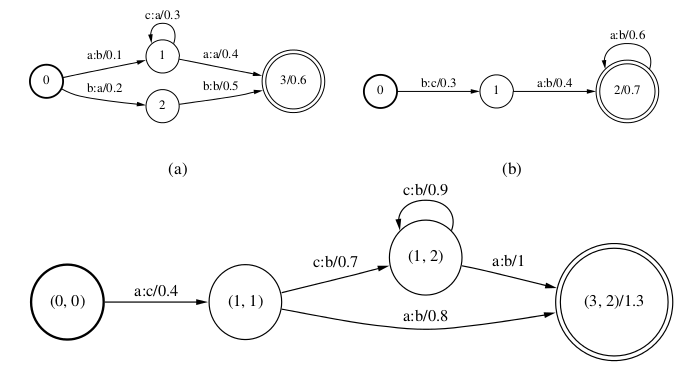
\includegraphics[width=8cm]{composition-example-0.png}  
\end{frame}

\begin{frame}
  \frametitle{Empty transitions}

  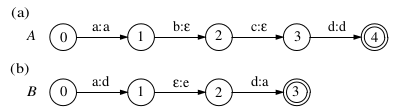
\includegraphics[width=5cm]{composition-example-1.png}\\
  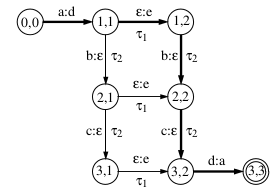
\includegraphics[width=4cm]{composition-example-2.png}

  Problem: weights assigned to output strings will be off --- loss of
  equivalence.
\end{frame}
\begin{frame}
  \frametitle{Empty transitions (cont.)}

  Solution: modify the source transducers, insert a filter:
  $$
  T_1 \circ T_2 = T'_1 \circ F \circ T'_2
  $$

  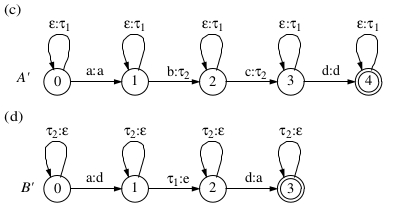
\includegraphics[width=5cm]{composition-example-3.png}
  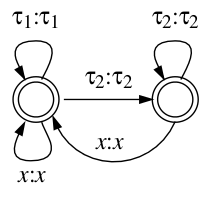
\includegraphics[width=3cm]{composition-example-4.png}
  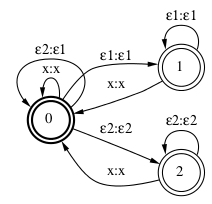
\includegraphics[width=3cm]{composition-example-5.png}
\end{frame}

\begin{frame}
  \frametitle{Composition}

  Complexity: worst case $|T_1| \cdot |T_2|$, much less in the typical
  ASR case.

  Algorithm can be performed lazily.
\end{frame}

\subsection{Determinization}
\begin{frame}
  \frametitle{Definition}
  
  A WSFT is {\em deterministic} iff
  \begin{itemize}
  \item there is exactly one initial state;
  \item every state has at most one outgoing transition for any given
    input label; and
  \item there are no input $\epsilon$-labels.
  \end{itemize}

  There is at most one path matching any given input string.
\end{frame}

\begin{frame}
  \frametitle{Algorithm}

  Mohri et al. only provide an algorithm for WFSA; we still have some
  questions on how to generalize it to WFST.

  A state in the result automaton is a {\em weighted subset} of
  states in the source WFSA: a set of pairs $\<q, x\>$ with $q \in Q$,
  $x \in \mathbb{K}$.

  A state $r$ of the result automaton that can be reached from the
  start state by path $\pi$ is the weighted set of pairs $\<q, x\>$
  such that $q$ can be reached from the initial state of the original
  automaton by a path $\sigma$ where $i[\sigma] = i[\pi]$, and 
  $\lambda[p[\sigma]] \otimes w[\sigma] = \lambda[p[\pi]] \otimes
  w[\pi] \otimes x$. ($x$ is the residual weight)
\end{frame}

\begin{frame}
  \frametitle{Example}

  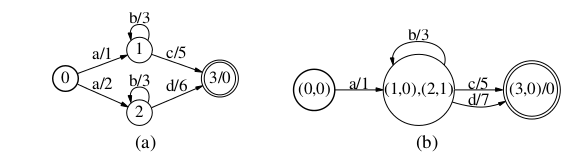
\includegraphics[width=8cm]{determinization-example.png}  
\end{frame}

\begin{frame}
  \frametitle{Complexity and stopping}
  
  Worst case complexity is exponential, but the blow-up does not occur
  in many practical cases.
  
  Can be computed lazily.

  No guarantee of stopping in the general case. The culprit: loops
  marked by the same path with different weight.

  % There are algoritms for {\em pre-determinization} by inserting new
  % transitions marked by special symbols.
\end{frame}

% \begin{frame}
%   Determinization produces a (usually) smaller transducer working from
%   the initial states forward. Minimization shrinks the WSFT working
%   backward from the final states.

%   Question: do we need determinization when there's minimization?
%   Laziness helps?
% \end{frame}

\subsection{Minimization}

\begin{frame}
  \frametitle{Minimization}

  Task: find a WSFT with the smallest number of nodes equivalent to a
  given WSFT $T$.

  General idea: merge nodes whose paths to the final state are
  identical.

  Problem: redistribution of weights along a path can mask similarity.
\end{frame}

\begin{frame}
  \frametitle{Weight pushing}

  Idea: define a potential function $V$ on $Q$. Modify transition
  weights\footnote{This assumes that your $\otimes$ operation is
    actually $+$.}:
  $$
  w'[t] = w[t] + V(n[t]) - V(p[t])
  $$
  Weights for final states:
  $$
  \rho[i] = \rho[i] + V(i) - V(f)
  $$
  The weight of each path remains the same.
\end{frame}

\begin{frame}
  \frametitle{Weight pushing for minimization}

  We should push weights as far as possible to the beginning of each
  path.

  Use the following potential function:
  $$
  d[q] = \bigoplus_{\pi \in P(q,F)} (w[\pi] \otimes \rho[n[\pi]])
  $$
  (the {\em shortest distance} from $q$ to $F$). Cheap to compute for
  the tropical semiring: $O(|E| + |Q|\log|Q|)$. Expensive for
  semirings like probability: $\Theta(|Q|^3(T_\oplus + T_\otimes + T_*))$.
\end{frame}

\begin{frame}
  \frametitle{Example}
  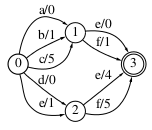
\includegraphics[width=4cm]{minimization-example-1.png}
  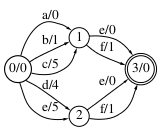
\includegraphics[width=4cm]{minimization-example-2.png}
%  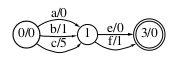
\includegraphics[width=4cm]{minimization-example-3.png}
$$
\begin{xy}
  \entrymodifiers={++[o][F-]}
  \xymatrix@C=2cm{
    {0/0} \ar@/^5ex/[r]^{a/0} \ar@/^2.5ex/[r]^{b/1} \ar[r]^{c/5} \ar@/_2.5ex/[r]^{d/4} \ar@/_5ex/[r]^{e/5} & 
    {1} \ar[r]^{e/0} \ar@/_2.5ex/[r]^{f/1} & 
    {3/0}
  }
\end{xy}
$$
\end{frame}

\begin{frame}
  \frametitle{Complexity}
  
  Computing the shortest distance: see above.

  Minimization itself: $O(|Q| + |E|)$ for the acyclic case,
  $O(|E|\log|Q|)$ for the general case.

  Does {\em not} appear to lend itself to lazy computation.
\end{frame}

\section{WFST use algorithms}

\begin{frame}
  \begin{itemize}
  \item Viterbi
  \end{itemize}
\end{frame}

\begin{frame}
  \frametitle{References}
  \begin{enumerate}
  \item Mori,~M., F.~Pereira, and M.~Riley. Speech Recognition with
    Weighted Finite-State Transducers. \textit{Handbook on Speech
      Processing and Speech Communication, Part E: Speech
      recognition}, 
    Springer-Verlag, Heidelberg, Germany (2008)
  \item Pereira,~F., and M.~Riley. \textit{ Speech Recognition by
      Composition of Weighted Finite Automata}. Finite-State
    Language Processing, MIT Press, Cambridge, Massachusetts (1997),
    pp. 431--453  
  \end{enumerate}
\end{frame}

\end{document}